% LSQR recursion follows Paige and Saunders, ACM TOMS 8 (1982), Algorithm LSQR.
% LSMR recursion checked against Fong and Saunders, SIAM J. Sci. Comput. 33 (2011), Algorithm LSMR.
\section{Golub--Kahan双对角化}
\label{sec:ls-bidiagonal-iteration}

\subsection{主要思想}

对一般的$\bm A\in\mathbb R^{m\times d}$，残差在$m$维的数据空间，未知量在$d$维空间，不能像方阵那样反复乘$\bm A$；把数据空间的向量送回未知量空间的是$\bm A^\top$。\term{Golub--Kahan双对角化}（Golub--Kahan bidiagonalization）因此交替作用$\bm A$与$\bm A^\top$，在数据空间建立标准正交基$\bm u_1,\bm u_2,\ldots$，在未知量空间建立与之配对的标准正交基$\bm v_1,\bm v_2,\ldots$。两组向量属于不同的空间，不能放进同一个正交化序列，只能各自在本空间内正交。

递推从右端开始。令$\beta_1=\lVert\bm b\rVert_2$、$\bm u_1=\bm b/\beta_1$，把$\bm A^\top\bm u_1$归一化为$\alpha_1\bm v_1$。已有$\bm u_k,\bm v_k$时，先把$\bm v_k$送到数据空间，从$\bm A\bm v_k$中扣除已经由$\bm u_k$解释的分量$\alpha_k\bm u_k$，令$\beta_{k+1}\bm u_{k+1}=\bm A\bm v_k-\alpha_k\bm u_k$；再把$\bm u_{k+1}$送回未知量空间，从$\bm A^\top\bm u_{k+1}$中扣除$\beta_{k+1}\bm v_k$，令$\alpha_{k+1}\bm v_{k+1}=\bm A^\top\bm u_{k+1}-\beta_{k+1}\bm v_k$。两次的系数都取余项的长度。

扣除的系数正是已经算出的$\alpha_k$与$\beta_{k+1}$：由$\bm A^\top\bm u_k=\beta_k\bm v_{k-1}+\alpha_k\bm v_k$，$\bm u_k^\top\bm A\bm v_k=\alpha_k$；由$\bm A\bm v_k=\alpha_k\bm u_k+\beta_{k+1}\bm u_{k+1}$，$\bm v_k^\top\bm A^\top\bm u_{k+1}=\beta_{k+1}$。每步只扣除一项而仍保持全部正交性，由下面的定理~\ref{thm:ls-golub-kahan-relations}用归纳证明。

把这些关系汇总，得到$\bm A\bm V_k=\bm U_{k+1}\bm B_k$，其中$\bm B_k$是对角元为$\alpha_1,\ldots,\alpha_k$、次对角元为$\beta_2,\ldots,\beta_{k+1}$的$(k+1)\times k$下双对角矩阵；转置方向则是$\bm A^\top\bm U_{k+1}=\bm V_k\bm B_k^\top+\alpha_{k+1}\bm v_{k+1}\bm e_{k+1}^\top$。后一式的边界项来自最后一个$\bm u_{k+1}$被$\bm A^\top$送回时产生的新方向，不能漏掉；若$\alpha_{k+1}=0$，这一项直接为零，也不引入$\bm v_{k+1}$。在这两组基下，长方矩阵问题被压缩成一个双对角的小问题。

两条作用关系相接，$\bm v_{k+1}$由$\bm A^\top\bm A\bm v_k$减去$\bm v_k,\bm v_{k-1}$的组合得到，所以右侧基张成$\mathcal K_k(\bm A^\top\bm A,\bm A^\top\bm b)$。实际计算只用$\bm A\bm v$与$\bm A^\top\bm u$，不形成$\bm A^\top\bm A$；有限精度下可按正交性的需要补做重正交化。它是后面LSQR和LSMR共用的内部过程，基向量和双对角系数只是求解器的中间状态，不作为输出。

\subsection{算法实现}

\paragraph{起步}
输入仍是$\bm A$与$\bm b\in\mathbb R^m$。后面两种求解器都固定零初值$\bm x_0=\bm0$，这是本节选出最小范数解的约定；生成多少步由求解器的步数上限$K$控制。起步先处理右端：若$\bm b=\bm0$，零向量满足方程，也是最小范数解，直接输出。否则令
\[
 \beta_1=\lVert\bm b\rVert_2,\quad \bm u_1=\bm b/\beta_1,\quad
 \bm q=\bm A^\top\bm u_1,\quad \alpha_1=\lVert\bm q\rVert_2 .
\]
若$\alpha_1=0$，则$\bm A^\top\bm b=\bm0$，零向量已满足正规方程\eqref{eq:linear-algebra-normal-equations}，同样直接输出；其余情况令$\bm v_1=\bm q/\alpha_1$。

\paragraph{交替扩展两组基}
然后逐轮扩展两组基。第$k$轮先把当前的未知量方向$\bm v_k$送到数据空间，减去它在$\bm u_k$上的分量并归一化；再把得到的$\bm u_{k+1}$送回未知量空间，减去它在$\bm v_k$上的分量并归一化：
\[
 \begin{aligned}
 \bm p&=\bm A\bm v_k-\alpha_k\bm u_k, & \beta_{k+1}&=\lVert\bm p\rVert_2,\\
 \bm q&=\bm A^\top\bm u_{k+1}-\beta_{k+1}\bm v_k, & \alpha_{k+1}&=\lVert\bm q\rVert_2,
 \end{aligned}
\]
其中$\beta_{k+1}\ne0$时$\bm u_{k+1}=\bm p/\beta_{k+1}$，$\alpha_{k+1}\ne0$时$\bm v_{k+1}=\bm q/\alpha_{k+1}$。减去的系数正是已经算出的$\alpha_k$和$\beta_{k+1}$，不需要另算内积；两次归一化分别发生在数据空间和未知量空间，所得长度就是新的双对角系数。

\paragraph{零系数的处理}
最后处理零系数。若$\beta_{k+1}=0$，无法生成$\bm u_{k+1}$，这时约定$\alpha_{k+1}=0$并停止生成；若$\beta_{k+1}>0$而$\alpha_{k+1}=0$，则不生成$\bm v_{k+1}$，转置关系中的边界项按零处理。两种情况下，本轮已经取得的系数仍交给LSQR或LSMR完成旋转与解的更新，然后检查目标并结束求解，不在当前小问题解完之前提前返回。近零的系数用与数据尺度相配的阈值判断；基停止扩张也不等于原残差为零，不相容问题的原残差可以停在非零值上。

\begin{example}[直线拟合上的两步双对角化]
\label{ex:ls-golub-kahan-line}
沿用示例~\ref{ex:ls-line-least-squares}的$\bm A=\left[\begin{smallmatrix}1&0\\1&1\\1&2\end{smallmatrix}\right]$与$\bm b=(1,2,2)^\top$。起步得$\beta_1=3$、$\bm u_1=(1,2,2)^\top/3$；$\bm A^\top\bm u_1=(5/3,2)^\top$，故$\alpha_1=\sqrt{61}/3\approx2.6034$，$\bm v_1=(5,6)^\top/\sqrt{61}$。

第一轮先把$\bm v_1$送到数据空间并扣除$\alpha_1\bm u_1$：
\[
 \begin{gathered}
 \bm A\bm v_1=\frac{(5,11,17)^\top}{\sqrt{61}},\\
 \bm p=\bm A\bm v_1-\alpha_1\bm u_1=\frac{(-16,-23,31)^\top}{9\sqrt{61}},
 \end{gathered}
\]
于是$\beta_2\approx0.5944$，$\bm u_2\approx(-0.3829,-0.5504,0.7419)^\top$；再由$\bm A^\top\bm u_2-\beta_2\bm v_1$得$\alpha_2\approx0.7446$，$\bm v_2=(-6,5)^\top/\sqrt{61}$。第二轮得$\beta_3\approx0.5607$，$\bm u_3\approx(-0.8615,0.5026,-0.0718)^\top$，而$\bm A^\top\bm u_3-\beta_3\bm v_2=\bm0$，即$\alpha_3=0$：未知量空间只有二维，已被$\bm v_1,\bm v_2$取尽，生成到此为止。

核对：$\bm u_1,\bm u_2,\bm u_3$两两正交；$\bm V_2$是正交方阵，$\bm A=\bm U_3\bm B_2\bm V_2^\top$，所以$\bm B_2^\top\bm B_2$与$\bm A^\top\bm A=\left[\begin{smallmatrix}3&3\\3&5\end{smallmatrix}\right]$有相同的迹$8$和行列式$6$。数值上
\[
 \begin{gathered}
 \alpha_1^2+\beta_2^2+\alpha_2^2+\beta_3^2\approx8.000,\\
 \alpha_1^2\alpha_2^2+\alpha_1^2\beta_3^2+\beta_2^2\beta_3^2\approx6.000 .
 \end{gathered}
\]
两个不变量都吻合。这项核对只用到双对角系数本身，不必重新比较各个基向量。
\end{example}

直线拟合的数据可以拟合到只剩一个非零的最优残差。下面换一个更简单的不相容系统，它的系数都有封闭形式，后面LSQR与LSMR的对照都用它作输入。

\begin{example}[不相容矩形系统上的双对角化]
\label{ex:ls-golub-kahan-diagonal}
取$\bm A=\left[\begin{smallmatrix}1&0\\0&2\\0&0\end{smallmatrix}\right]$，$\bm b=(1,1,1)^\top$。第三行恒为零，$\bm b$的第三个分量无法拟合，最小二乘解是$\hat{\bm x}=(1,1/2)^\top$，最优残差为$(0,0,1)^\top$。起步得$\beta_1=\sqrt3$，$\bm u_1=(1,1,1)^\top/\sqrt3$；$\bm A^\top\bm u_1=(1,2)^\top/\sqrt3$，故$\alpha_1=\sqrt{5/3}$，$\bm v_1=(1,2)^\top/\sqrt5$。

第一轮$\bm A\bm v_1=(1,4,0)^\top/\sqrt5$，扣除$\alpha_1\bm u_1=\sqrt5(1,1,1)^\top/3$得
\[
 \bm A\bm v_1-\alpha_1\bm u_1=\frac{(-2,7,-5)^\top}{3\sqrt5},
\]
故$\beta_2=\sqrt{78}/(3\sqrt5)$，$\bm u_2=(-2,7,-5)^\top/\sqrt{78}$。再由$\bm A^\top\bm u_2=(-2,14)^\top/\sqrt{78}$扣除$\beta_2\bm v_1=\sqrt{78}(1,2)^\top/15$，得$18(-2,1)^\top/(5\sqrt{78})$，因此$\alpha_2=18\sqrt5/(5\sqrt{78})$，$\bm v_2=(-2,1)^\top/\sqrt5$。

第二轮$\bm A\bm v_2-\alpha_2\bm u_2=5(-4,1,3)^\top/(13\sqrt5)$，得$\beta_3=\sqrt{10/13}$，$\bm u_3=(-4,1,3)^\top/\sqrt{26}$；而$\bm A^\top\bm u_3=(-4,2)^\top/\sqrt{26}$恰好等于$\beta_3\bm v_2$，所以$\alpha_3=0$。逐列核验$\bm A\bm V_2=\bm U_3\bm B_2$：第一列$\alpha_1\bm u_1+\beta_2\bm u_2=(1,4,0)^\top/\sqrt5=\bm A\bm v_1$，第二列同理。右侧二维空间已经生成完毕，但$\bm b$在第三行的分量仍不可拟合，原残差不会降到零。
\end{example}

\subsection{算法分析}

\paragraph{正确性}
把前$k$轮的系数排成$(k+1)\times k$的下双对角矩阵，并记$\bm U_{k+1}=[\bm u_1\;\cdots\;\bm u_{k+1}]$、$\bm V_k=[\bm v_1\;\cdots\;\bm v_k]$：
\[
 \bm B_k=
 \begin{bmatrix}
 \alpha_1&&&\\
 \beta_2&\alpha_2&&\\
 &\beta_3&\ddots&\\
 &&\ddots&\alpha_k\\
 &&&\beta_{k+1}
 \end{bmatrix}.
\]
下面的定理说明，短递推得到的两组基确实标准正交，并把递推整理成矩阵关系。

\begin{theorem}[Golub--Kahan关系]
\label{thm:ls-golub-kahan-relations}
设$\alpha_1,\ldots,\alpha_k$与$\beta_2,\ldots,\beta_{k+1}$都为正。则在精确算术中，$\bm U_{k+1}$与$\bm V_k$的列分别标准正交，
\begin{equation}
 \bm A\bm V_k=\bm U_{k+1}\bm B_k,\qquad
 \bm A^\top\bm U_{k+1}=\bm V_k\bm B_k^\top+\alpha_{k+1}\bm v_{k+1}\bm e_{k+1}^\top,
 \label{eq:ls-golub-kahan-relations}
\end{equation}
其中$\alpha_{k+1}=0$时末项为零；并且$\operatorname{range}(\bm V_k)=\mathcal K_k(\bm A^\top\bm A,\bm A^\top\bm b)$。
\end{theorem}

\begin{proof}
由$\bm p,\bm q$的定义，$\bm A\bm v_i=\alpha_i\bm u_i+\beta_{i+1}\bm u_{i+1}$，$\bm A^\top\bm u_i=\beta_i\bm v_{i-1}+\alpha_i\bm v_i$（约定$\bm v_0=\bm0$），它们分别是\eqref{eq:ls-golub-kahan-relations}两式的第$i$列。正交性对$k$归纳。设$\bm u_1,\ldots,\bm u_k$与$\bm v_1,\ldots,\bm v_k$已分别标准正交，对$j\le k$，由这两个列关系，
\[
 \begin{aligned}
 \beta_{k+1}\bm u_j^\top\bm u_{k+1}
 &=\bm v_k^\top\bm A^\top\bm u_j-\alpha_k\bm u_j^\top\bm u_k\\
 &=\bm v_k^\top(\beta_j\bm v_{j-1}+\alpha_j\bm v_j)-\alpha_k\delta_{j,k}=0 .
 \end{aligned}
\]
同理，由关系$\bm A\bm v_j=\alpha_j\bm u_j+\beta_{j+1}\bm u_{j+1}$以及刚证明的$\bm u$的正交性，$\alpha_{k+1}\bm v_j^\top\bm v_{k+1}=\beta_{j+1}\delta_{j,k}-\beta_{k+1}\delta_{j,k}=0$。最后，$\bm v_1\parallel\bm A^\top\bm b$，而$\bm v_{i+1}$由$\bm A^\top\bm A\bm v_i$减去$\bm v_i,\bm v_{i-1}$的组合得到，归纳可知$\bm v_i\in\mathcal K_i(\bm A^\top\bm A,\bm A^\top\bm b)$。$\bm V_k$的$k$列标准正交，而该Krylov空间至多$k$维，两者相等。
\end{proof}

因此零初值下双对角化生成的正是第~\ref{sec:ls-krylov-subspaces}节所说的长方矩阵Krylov空间，但从不形成$\bm A^\top\bm A$。生成终止时，把未生成的基向量连同它的零系数从\eqref{eq:ls-golub-kahan-relations}中略去，两式仍成立。图~\ref{fig:ls-golub-kahan-bidiagonal}把递推与矩阵关系放在一起：(a)中进出$\bm v_i$的两支箭头给出$\alpha_i$与$\beta_{i+1}$，它们正是(b)中$\bm B_k$的第$i$列；每个新向量只与对面空间中相邻的一个向量相连，这就是每步只需扣除一项的原因。

\begin{figure}[htbp]
  \centering
  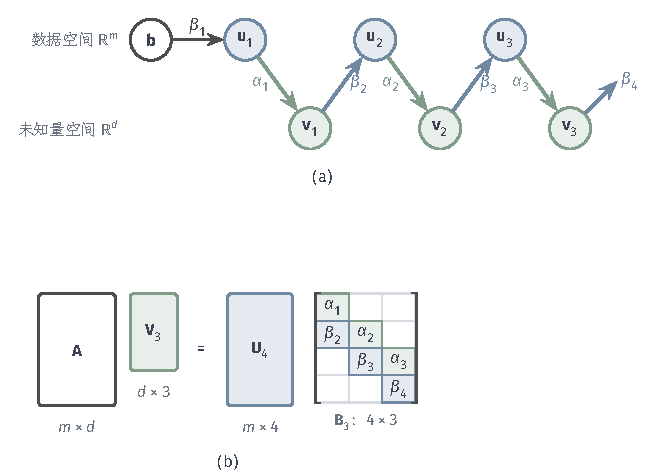
\includegraphics[width=109.343mm]{figures/01-basic-mathematics/03-vectors-matrices-and-multivariate-functions/tikz/c5-golub-kahan-bidiagonal/figure.pdf}
  \caption{Golub--Kahan双对角化的递推与矩阵关系（$k=3$）。(a)蓝色$\bm u_i$在数据空间，绿色$\bm v_i$在未知量空间；乘$\bm A^\top$并扣除前一个$\bm v$后归一化得到$\bm v_i$，长度为$\alpha_i$，乘$\bm A$并扣除前一个$\bm u$后归一化得到$\bm u_{i+1}$，长度为$\beta_{i+1}$。(b)这些长度排成$4\times3$的下双对角矩阵$\bm B_3$，满足$\bm A\bm V_3=\bm U_4\bm B_3$；绿格为对角元，蓝格为次对角元，其余元素为零。}
  \label{fig:ls-golub-kahan-bidiagonal}
\end{figure}

\paragraph{数值稳定性}
在浮点运算中，正交性所依赖的相消只近似成立，短递推也不会去掉舍入引入的旧方向分量，两组基会逐渐失去正交性；它对求解结果的影响交给两种求解器，由第~\ref{sec:ls-krylov-stopping}节的真实残差复核来控制，必要时以保存基并重正交化的代价换取正交性。

\paragraph{计算代价}
每轮至多一次$\bm A$乘向量和一次$\bm A^\top$乘向量，外加两次向量更新、两次范数和两次缩放。LSQR与LSMR只用当前的$\bm u_k,\bm v_k$，不保存整组基、不作完整再正交化时，工作存储为$O(m+d)$。双对角化只负责生成候选空间，收敛快慢取决于下一步在子空间中怎样选取近似解。

\section{LSQR算法}
\label{sec:ls-lsqr}

\subsection{主要思想}

LSQR由Paige与Saunders提出\scite{math-paige1982lsqr}，它在$\operatorname{range}(\bm V_k)$中直接最小化原残差。令$\bm x=\bm V_k\bm y$，由$\bm b=\beta_1\bm u_1=\bm U_{k+1}\beta_1\bm e_1$和\eqref{eq:ls-golub-kahan-relations}，
\[
 \bm b-\bm A\bm V_k\bm y=\bm U_{k+1}(\beta_1\bm e_1-\bm B_k\bm y).
\]
$\bm U_{k+1}$的列标准正交，不改变长度，所以第$k$步只需解一个$(k+1)\times k$的双对角最小二乘问题：
\begin{equation}
 \bm x_k=\bm V_k\bm y_k,\qquad
 \bm y_k=\argmin_{\bm y\in\mathbb R^k}\lVert\beta_1\bm e_1-\bm B_k\bm y\rVert_2 .
 \label{eq:ls-lsqr-subproblem}
\end{equation}
这一做法不要求$\bm A$是方阵、满秩或相容，相容方程与不相容最小二乘问题都适用。

小问题的QR分解可以逐列延续。设前$k-1$列已化为上三角，第$k$、$k+1$两行待处理的是第$k$列的$(\bar\rho_k,\beta_{k+1})$、新的第$k+1$列的$(0,\alpha_{k+1})$和右端的$(\bar\phi_k,0)$。取$\rho_k=\operatorname{hypot}(\bar\rho_k,\beta_{k+1})$、$c_k=\bar\rho_k/\rho_k$、$s_k=\beta_{k+1}/\rho_k$，把对称的正交变换$\left[\begin{smallmatrix}c_k&s_k\\s_k&-c_k\end{smallmatrix}\right]$作用于这两行：
\[
 \begin{bmatrix}c_k&s_k\\s_k&-c_k\end{bmatrix}
 \begin{bmatrix}\bar\rho_k&0&\bar\phi_k\\\beta_{k+1}&\alpha_{k+1}&0\end{bmatrix}
 =\begin{bmatrix}\rho_k&\theta_{k+1}&\phi_k\\0&\bar\rho_{k+1}&\bar\phi_{k+1}\end{bmatrix},
\]
其中$\theta_{k+1}=s_k\alpha_{k+1}$、$\bar\rho_{k+1}=-c_k\alpha_{k+1}$、$\phi_k=c_k\bar\phi_k$、$\bar\phi_{k+1}=s_k\bar\phi_k$。左下角为$s_k\bar\rho_k-c_k\beta_{k+1}=0$，所以$\beta_{k+1}$被消去。这是Paige与Saunders原文的反射式约定；它与第~\ref{sec:ls-gmres}节的旋转只差第二行的符号，$\bar\rho_{k+1}$与$\bar\phi_{k+1}$随之变号，各量的绝对值和后面的残差估计都不变。

所得上三角因子$\bm R_k$只有对角元$\rho_1,\ldots,\rho_k$与上副对角元$\theta_2,\ldots,\theta_k$，解因此可以逐列递推。记$\bm V_k\bm R_k^{-1}$的第$i$列为$\bm w_i/\rho_i$，比较$(\bm V_k\bm R_k^{-1})\bm R_k=\bm V_k$的第$i+1$列，得$\theta_{i+1}\bm w_i/\rho_i+\bm w_{i+1}=\bm v_{i+1}$，即
\[
 \bm w_1=\bm v_1,\qquad \bm w_{k+1}=\bm v_{k+1}-\frac{\theta_{k+1}}{\rho_k}\bm w_k .
\]
小问题的解是$\bm y_k=\bm R_k^{-1}(\phi_1,\ldots,\phi_k)^\top$，于是$\bm x_k=\sum_{i\le k}(\phi_i/\rho_i)\bm w_i$，已确定的$\phi_i$此后不变，回代化为逐步累加$\bm x_k=\bm x_{k-1}+(\phi_k/\rho_k)\bm w_k$。

这一短递推与完整的小问题回代给出同一个$\bm x_k$，却只保存一个方向。变换后右端的末分量$\lvert\bar\phi_{k+1}\rvert$就是原残差长度，提供了不必形成残差的停止估计；有限精度下它会偏离真实值，仍须直接重算原残差和正规残差来核验。

\subsection{算法实现}

\paragraph{初始化}
LSQR的输入是一般的实矩阵$\bm A$与$\bm b$，允许秩亏，输出为$\bm x$。超参数是阈值和步数上限$K$：以最小二乘为目标时，用正规残差的绝对阈值$\tau_n\ge0$；以相容方程为目标时，另用第~\ref{sec:ls-stationary-stopping}节的$\mathrm{atol},\mathrm{rtol}$。初值固定为$\bm x_0=\bm0$。若$K=0$，直接输出$\bm x_0$；否则先按第~\ref{sec:ls-bidiagonal-iteration}节的起步检查零右端与已满足正规方程的情形，并按第~\ref{sec:ls-krylov-stopping}节检查初值。初值的原残差是$\bm b$，正规残差$\bm A^\top\bm b$的长度是$\alpha_1\beta_1$，这一检查与双对角化的起步共用同一次$\bm A^\top$乘法。初值已满足条件或起步给出零解时输出$\bm x_0$，否则取
\[
 \bm w_1=\bm v_1,\qquad \bar\rho_1=\alpha_1,\qquad \bar\phi_1=\beta_1 .
\]
这里$\bar\rho_1$是小问题第一列尚未变换的对角元，$\bar\phi_1$是右端$\beta_1\bm e_1$的第一个分量，$\bm w_1$是第一个更新方向。

\paragraph{双对角化与正交变换}
第$k$轮先做一次双对角化，得到$\beta_{k+1},\alpha_{k+1}$及存在的$\bm u_{k+1},\bm v_{k+1}$；扩张停止时跳过不存在的新基，本轮的变换照常完成。然后按主要思想中的公式依次计算
\[
 \begin{gathered}
 \rho_k=\sqrt{\bar\rho_k^2+\beta_{k+1}^2},\qquad
 c_k=\frac{\bar\rho_k}{\rho_k},\qquad s_k=\frac{\beta_{k+1}}{\rho_k},\\
 \theta_{k+1}=s_k\alpha_{k+1},\qquad
 \bar\rho_{k+1}=-c_k\alpha_{k+1},\\
 \phi_k=c_k\bar\phi_k,\qquad
 \bar\phi_{k+1}=s_k\bar\phi_k .
 \end{gathered}
\]
其中$\rho_k$与$\theta_{k+1}$是上双对角因子$\bm R_k$的新对角元和上对角元，$\phi_k$是变换后右端的第$k$个分量，$\bar\rho_{k+1}$与$\bar\phi_{k+1}$留给下一轮。

\paragraph{更新解与停止}
变换完成后，用当前方向更新解：
\[
 \bm x_k=\bm x_{k-1}+\frac{\phi_k}{\rho_k}\bm w_k .
\]
这时原残差与正规残差的长度可以直接从标量读出，分别为$|\bar\phi_{k+1}|$和$|\bar\phi_{k+1}|\alpha_{k+1}|c_k|$。若相应的估计达到第~\ref{sec:ls-krylov-stopping}节的阈值，或已达到$K$，就按该节复核后输出$\bm x_k$；否则取下一方向$\bm w_{k+1}=\bm v_{k+1}-(\theta_{k+1}/\rho_k)\bm w_k$，进入下一轮。$\bm w_{k+1}$排在$\bm x_k$之后计算，因为两者都要用旧的$\bm w_k$。

\paragraph{零系数与异常}
双对角化出现零系数时，本轮的变换和解更新照常完成，之后不再生成下一方向，直接计算$\bm r=\bm b-\bm A\bm x_k$与$\bm A^\top\bm r$，按相容方程或一般最小二乘分别验收：$\beta_{k+1}=0$使$s_k=0$，原残差估计为零；$\alpha_{k+1}=0$使正规残差估计为零。正常步骤中$\rho_k>0$：$\bar\rho_1=\alpha_1>0$，而只要继续迭代就有$\alpha_{k+1}>0$，归纳可知各$\bar\rho_k\ne0$，所以$\rho_k\ge|\bar\rho_k|>0$。出现零$\rho_k$、明显失去正交性、到达迭代上限或残差长期不降时，分别报告不同的原因，不把残差估计当成无需复核的精确值。

\begin{example}[直线拟合上的LSQR]
\label{ex:ls-lsqr-line}
沿用示例~\ref{ex:ls-golub-kahan-line}的系数。初始化取$\bm w_1=\bm v_1$、$\bar\rho_1=\alpha_1\approx2.6034$、$\bar\phi_1=3$。第一轮的变换由$(\bar\rho_1,\beta_2)\approx(2.6034,0.5944)$得$\rho_1\approx2.6704$、$c_1\approx0.9749$、$s_1\approx0.2226$；作用于新列和右端，得$\theta_2\approx0.1658$、$\bar\rho_2\approx-0.7259$、$\phi_1\approx2.9247$、$\bar\phi_2\approx0.6678$。更新解得
\[
 \bm x_1=\frac{\phi_1}{\rho_1}\bm w_1=\frac{61}{435}(5,6)^\top\approx(0.7011,0.8414)^\top ,
\]
它是沿$\bm A^\top\bm b=(5,6)^\top$方向使残差最小的点。两个估计$|\bar\phi_2|\approx0.6678$和$|\bar\phi_2|\alpha_2|c_1|\approx0.4848$与直接计算的$\lVert\bm b-\bm A\bm x_1\rVert_2=\sqrt{194/435}$和$\lVert\bm A^\top(\bm b-\bm A\bm x_1)\rVert_2$一致。

由于$\alpha_3=0$，第二轮完成变换和更新后结束：$\rho_2\approx0.9173$、$\phi_2\approx-0.5285$，$\bm w_2=\bm v_2-(\theta_2/\rho_1)\bm w_1\approx(-0.8080,0.5925)^\top$，$\bm x_2=\bm x_1+(\phi_2/\rho_2)\bm w_2=(7/6,1/2)^\top$，正是最小二乘解$\hat{\bm x}$；原残差估计$|\bar\phi_3|\approx0.4082=1/\sqrt6$等于最优残差$(-1/6,1/3,-1/6)^\top$的长度，正规残差估计为零。
\end{example}

\begin{example}[不相容矩形系统上的LSQR]
\label{ex:ls-lsqr-diagonal}
沿用示例~\ref{ex:ls-golub-kahan-diagonal}的系数，初始化$\bar\rho_1=\alpha_1=\sqrt{5/3}$、$\bar\phi_1=\sqrt3$。第一轮$\rho_1=\sqrt{\alpha_1^2+\beta_2^2}=\sqrt{17/5}\approx1.8439$，$c_1=5/\sqrt{51}$，$s_1=\sqrt{26/51}$，于是$\theta_2=6/\sqrt{85}$、$\bar\rho_2=-\sqrt{90/221}$、$\phi_1=5/\sqrt{17}$、$\bar\phi_2=\sqrt{26/17}$。更新得
\[
 \bm x_1=\frac{\phi_1}{\rho_1}\bm v_1=\frac5{17}(1,2)^\top .
\]
直接计算$\bm r_1=\bm b-\bm A\bm x_1=(12/17,-3/17,1)^\top$，长度$\sqrt{26/17}=\lvert\bar\phi_2\rvert$；正规残差$\bm A^\top\bm r_1=(12/17,-6/17)^\top$，长度约$0.7892$，与$\lvert\bar\phi_2\rvert\alpha_2\lvert c_1\rvert$一致。

第二轮保留第一轮的方向与标量：$\rho_2=\sqrt{\bar\rho_2^2+\beta_3^2}=\sqrt{20/17}\approx1.084652289$，$c_2=-3/\sqrt{26}$，$\phi_2=c_2\bar\phi_2=-3/\sqrt{17}\approx-0.727606875$，$\bar\phi_3=1$；由于$\alpha_3=0$，$\theta_3=\bar\rho_3=0$。方向$\bm w_2=\bm v_2-(\theta_2/\rho_1)\bm w_1=\bm v_2-\tfrac6{17}\bm v_1=(-40,5)^\top/(17\sqrt5)$，于是
\[
 \bm x_2=\bm x_1+\frac{\phi_2}{\rho_2}\bm w_2=\Bigl(1,\frac12\Bigr)^\top .
\]
这时$\bm r_2=(0,0,1)^\top$，$\bm A^\top\bm r_2=\bm0$：最小二乘已经完成，原残差停在不可拟合的长度$1=\lvert\bar\phi_3\rvert$上。独立复核：小问题$\min\lVert\beta_1\bm e_1-\bm B_2\bm y\rVert_2$的正规方程是$\bm B_2^\top\bm B_2\bm y=\alpha_1\beta_1\bm e_1$，解出的$\bm V_2\bm y$同样是$(1,1/2)^\top$。
\end{example}

\subsection{算法分析}

\paragraph{正确性}
先说明递推确实解出了小问题\eqref{eq:ls-lsqr-subproblem}。

\begin{theorem}[LSQR递推的正确性]
\label{thm:ls-lsqr-recursion}
在精确算术中，设双对角化在第$k$轮之前没有终止。则按上述递推得到的$\bm x_k$等于$\bm V_k\bm y_k$，其中$\bm y_k$是小问题\eqref{eq:ls-lsqr-subproblem}的解，即$\bm x_k$是$\operatorname{range}(\bm V_k)$中使$\lVert\bm b-\bm A\bm x\rVert_2$最小的点；并且
\[
 \lVert\bm r_k\rVert_2=|\bar\phi_{k+1}|,\qquad
 \lVert\bm A^\top\bm r_k\rVert_2=|\bar\phi_{k+1}|\,\alpha_{k+1}|c_k| .
\]
\end{theorem}

\begin{proof}
记前$k$次正交变换之积为$\bm Q_k$。每轮的新列只在第$k$、$k+1$行非零，此前的变换都不触及它的第$k+1$行，所以一次新变换就能延续三角化，归纳得到
\[
 \bm Q_k\begin{bmatrix}\bm B_k&\beta_1\bm e_1\end{bmatrix}
 =\begin{bmatrix}\bm R_k&\bm f_k\\ \bm0^\top&\bar\phi_{k+1}\end{bmatrix},
\]
其中$\bm R_k$上双对角，对角元为$\rho_1,\ldots,\rho_k$，上对角元为$\theta_2,\ldots,\theta_k$，$\bm f_k=(\phi_1,\ldots,\phi_k)^\top$。$\bm Q_k$正交，所以$\lVert\beta_1\bm e_1-\bm B_k\bm y\rVert_2^2=\lVert\bm f_k-\bm R_k\bm y\rVert_2^2+\bar\phi_{k+1}^2$，最小点是$\bm y_k=\bm R_k^{-1}\bm f_k$，最小残差$|\bar\phi_{k+1}|$就是$\lVert\bm r_k\rVert_2$。主要思想中已由$(\bm V_k\bm R_k^{-1})\bm R_k=\bm V_k$逐列推出方向递推；$\bm R_k$和$\bm f_k$在后续轮次中不再改动，回代因此化为逐步累加$\bm x_k=\bm x_{k-1}+\phi_k\bm w_k/\rho_k$。正规残差估计来自\eqref{eq:ls-golub-kahan-relations}的第二式：小问题的残差$\bm g_k=\beta_1\bm e_1-\bm B_k\bm y_k$满足$\bm B_k^\top\bm g_k=\bm0$，所以$\bm A^\top\bm r_k=\alpha_{k+1}(\bm e_{k+1}^\top\bm g_k)\bm v_{k+1}$；而$\bm g_k=\bm Q_k^\top(\bm0,\bar\phi_{k+1})^\top$，只有最后一次变换触及第$k+1$个分量，得$\bm e_{k+1}^\top\bm g_k=-c_k\bar\phi_{k+1}$。
\end{proof}

\paragraph{残差的单调性与选出的解}
由此可以读出LSQR的几条性质。候选空间逐轮嵌套，所以精确算术中原残差不增；正规残差没有这样的保证，可能某一步上升。每个$\bm v_i$都由$\bm A^\top$作用后再作组合得到，零初值使各步近似都留在$\operatorname{range}(\bm A^\top)$中。一旦达到正规方程，$\bm x_k$就是与$\operatorname{null}(\bm A)$正交的最小二乘解，即第~\ref{sec:ls-pseudoinverse}节的$\bm A^\dagger\bm b$；$\alpha_{k+1}=0$正是这种情形。

\paragraph{与正规方程上CG的关系}
LSQR与正规方程上的CG还有下面的等价关系。

\begin{theorem}[LSQR与正规方程上的CG]
\label{thm:ls-lsqr-cg-equivalence}
在精确算术中，只要两种方法都尚未终止，LSQR的第$k$步近似就等于对正规方程$\bm A^\top\bm A\bm x=\bm A^\top\bm b$从$\bm x_0=\bm0$施行第~\ref{sec:ls-conjugate-gradient}节CG的第$k$步近似。
\end{theorem}

\begin{proof}
记$\hat{\bm x}=\bm A^\dagger\bm b$，$\hat{\bm r}=\bm b-\bm A\hat{\bm x}$。CG的各步都在$\mathcal K_k(\bm A^\top\bm A,\bm A^\top\bm b)\subseteq\operatorname{range}(\bm A^\top)$中，$\bm A^\top\bm A$在这个子空间上正定，所以CG的第$k$步是该Krylov空间中使$\lVert\bm x-\hat{\bm x}\rVert_{\bm A^\top\bm A}^2=\lVert\bm A(\bm x-\hat{\bm x})\rVert_2^2$最小的点。另一方面，$\hat{\bm r}$与$\operatorname{range}(\bm A)$正交，由勾股定理
\[
 \lVert\bm b-\bm A\bm x\rVert_2^2=\lVert\hat{\bm r}\rVert_2^2+\lVert\bm A(\bm x-\hat{\bm x})\rVert_2^2 ,
\]
右边第一项与$\bm x$无关。由定理~\ref{thm:ls-golub-kahan-relations}，两种方法的候选空间都是$\operatorname{range}(\bm V_k)$，最小化的又是同一个函数；$\bm A$在$\operatorname{range}(\bm A^\top)$上是单射，最小点唯一，所以两者相等。
\end{proof}

\paragraph{收敛速度与数值敏感度}
由这一等价，CG的收敛界可以直接搬到LSQR：迭代面对的是$\bm A^\top\bm A$，收敛快慢由$\bm A$的非零奇异值的平方的分布决定。$\bm A$满列秩时，$\kappa_2(\bm A^\top\bm A)=\kappa_2(\bm A)^2$，CG界中的$\sqrt{\kappa}$正好是$\kappa_2(\bm A)$，于是$\lVert\bm A(\bm x_k-\hat{\bm x})\rVert_2\le2\bigl((\kappa_2(\bm A)-1)/(\kappa_2(\bm A)+1)\bigr)^k\lVert\bm A\hat{\bm x}\rVert_2$。

LSQR不形成Gram矩阵，避免了第~\ref{sec:ls-normal-equations-method}节在形成$\bm A^\top\bm A$时丢失信息，但这并不消除原问题的病态性：$\kappa_2(\bm A)$很大时上式的因子仍接近$1$，问题对数据的敏感度也不因算法改变。有限精度下基的正交性和两个残差估计都会偏离精确值，仍须按第~\ref{sec:ls-krylov-stopping}节复核。

\paragraph{计算代价}
每轮的核心工作是一次$\bm A$乘向量和一次$\bm A^\top$乘向量，另加十几次标量运算、一次正交变换和两次长度为$d$的向量更新；需要保存的是$\bm u$和$\bm v,\bm w,\bm x$，工作存储为$O(m+d)$。对相容方程，LSQR也能求解，但每轮多一次转置作用，是否比方阵专用的方法划算，要结合矩阵结构与精度目标比较。

\section{LSMR算法}
\label{sec:ls-lsmr}

\subsection{主要思想}

LSMR由Fong与Saunders提出\scite{math-fong2011lsmr}。它与LSQR在同一个子空间$\operatorname{range}(\bm V_k)$中取点，但改为最小化正规残差$\lVert\bm A^\top(\bm b-\bm A\bm x)\rVert_2$，这正是判断是否到达最小二乘解所看的量。用$\bm A^\top$左乘原残差的表示$\bm U_{k+1}(\beta_1\bm e_1-\bm B_k\bm y)$，由\eqref{eq:ls-golub-kahan-relations}的第二式及$\bm B_k^\top\bm e_1=\alpha_1\bm e_1$、$\bm e_{k+1}^\top\bm B_k=\beta_{k+1}\bm e_k^\top$，得到
\begin{equation}
 \begin{gathered}
 \bm A^\top(\bm b-\bm A\bm V_k\bm y)
 =\bm V_{k+1}\bigl(\alpha_1\beta_1\bm e_1-\bm C_k\bm y\bigr),\\
 \bm C_k=\begin{bmatrix}\bm B_k^\top\bm B_k\\ \alpha_{k+1}\beta_{k+1}\bm e_k^\top\end{bmatrix}.
 \end{gathered}
 \label{eq:ls-lsmr-subproblem}
\end{equation}
$\bm V_{k+1}$的列标准正交，所以第$k$步求解小问题$\min_{\bm y}\lVert\alpha_1\beta_1\bm e_1-\bm C_k\bm y\rVert_2$，区别于LSQR最小化原残差。若$\alpha_{k+1}=0$，$\bm C_k$的最后一行为零，删去它并只用已有的$\bm V_k$表达，不假定存在额外的右基向量。

实际计算不形成$\bm B_k^\top\bm B_k$，否则又回到了Gram矩阵。先用LSQR的第一组正交变换把$\bm B_k$三角化为上双对角的$\bm R_k$，则$\bm B_k^\top\bm B_k=\bm R_k^\top\bm R_k$。令$\bm t=\bm R_k\bm y$；$\bm R_k^{-1}$是上三角矩阵，末行只有对角元$1/\rho_k$，所以$\bm e_k^\top\bm y=\bm e_k^\top\bm R_k^{-1}\bm t=t_k/\rho_k$。小问题于是改写为
\[
 \min_{\bm t}\Bigl\lVert\alpha_1\beta_1\bm e_1-\begin{bmatrix}\bm R_k^\top\\ \theta_{k+1}\bm e_k^\top\end{bmatrix}\bm t\Bigr\rVert_2,\qquad
 \theta_{k+1}=\frac{\alpha_{k+1}\beta_{k+1}}{\rho_k},
\]
这里的$\theta_{k+1}$与第一组变换给出的$s_k\alpha_{k+1}$相同。

增广矩阵是下双对角的，形状与$\bm B_k$一样，所以可以像LSQR那样再作一组正交变换，把它化为上双对角的$\bar{\bm R}_k$（对角元$\bar\rho_i$，上对角元$\bar\theta_{i+1}$），右端化为$\bm z_k=(\zeta_1,\ldots,\zeta_k)^\top$与末分量$\bar\zeta_{k+1}$。于是依次解$\bar{\bm R}_k\bm t=\bm z_k$与$\bm R_k\bm y=\bm t$，两组变换都只更新小矩阵的边界项，无需形成$\bm A^\top\bm A$。

两次三角求解对应两层方向。定义$\bm W_k\bm R_k=\bm V_k$与$\bar{\bm W}_k\bar{\bm R}_k=\bm W_k$，逐列展开得
\[
 \bm w_k=\frac{\bm v_k-\theta_k\bm w_{k-1}}{\rho_k},\qquad
 \bar{\bm w}_k=\frac{\bm w_k-\bar\theta_k\bar{\bm w}_{k-1}}{\bar\rho_k},\qquad
 \bm x_k=\bm x_{k-1}+\zeta_k\bar{\bm w}_k ,
\]
因为$\bm x_k=\bm V_k\bm R_k^{-1}\bar{\bm R}_k^{-1}\bm z_k=\bar{\bm W}_k\bm z_k$，而$\bm z_k$已确定的分量此后不变。$\rho,\theta$与$\bar\rho,\bar\theta$分别是两组三角因子的对角元和上副对角元。

\subsection{算法实现}

\paragraph{初始化}
输入、超参数、零初值和输出的约定都与LSQR相同。先按第~\ref{sec:ls-bidiagonal-iteration}节的起步检查零右端与已满足正规方程的情形，零解直接输出；否则取
\[
 \begin{gathered}
 \bm x_0=\bm0,\qquad \bm w_0=\bar{\bm w}_0=\bm0,\qquad \theta_1=0,\\
 \bar\alpha_1=\alpha_1,\qquad \bar\zeta_1=\alpha_1\beta_1,\qquad \bar c_0=1,\qquad \bar s_0=0 .
 \end{gathered}
\]
$\bar\zeta_1=\lVert\bm A^\top\bm b\rVert_2$是初始正规残差的长度；$\bar\alpha_1$相当于LSQR中的$\bar\rho_1$，改名是为了把带横线的$\rho$留给第二组变换。其余几个量只是占位，使第一轮的公式不必单独处理：$\theta_1=0$与$\bm w_0=\bm0$使$\bm w_1=\bm v_1/\rho_1$，$\bar s_0=0$使第一轮的$\bar\theta_1=0$。这里采用未缩放的方向，使它们与两次三角回代直接对应。

\paragraph{第一组旋转}
第$k$轮先完成一次双对角化，再作第一组旋转。本节使用第~\ref{sec:ls-gmres}节的旋转约定$\left[\begin{smallmatrix}c&s\\-s&c\end{smallmatrix}\right]$，它把$\bm B_k$化为与LSQR相同的上双对角因子$\bm R_k$，只是$\bar\alpha_{k+1}$与LSQR的$\bar\rho_{k+1}$差一个符号：
\[
 \begin{gathered}
 \rho_k=\sqrt{\bar\alpha_k^2+\beta_{k+1}^2},\qquad
 c_k=\frac{\bar\alpha_k}{\rho_k},\qquad s_k=\frac{\beta_{k+1}}{\rho_k},\\
 \theta_{k+1}=s_k\alpha_{k+1},\qquad
 \bar\alpha_{k+1}=c_k\alpha_{k+1}.
 \end{gathered}
\]

\paragraph{第二组旋转}
接着作第二组旋转。它处理的是对角元为$\rho_i$、下对角元为$\theta_{i+1}$的下双对角矩阵，新列在第$k$、$k+1$行上的元素是$\rho_k,\theta_{k+1}$。上一轮的旋转$(\bar c_{k-1},\bar s_{k-1})$先作用于这一列的第$k-1$、$k$行，在第$k-1$行产生$\bar\theta_k$，在第$k$行留下$\bar c_{k-1}\rho_k$；本轮旋转再消去它下方的$\theta_{k+1}$，并把右端分量$\bar\zeta_k$分成$\zeta_k$与留给下一轮的$\bar\zeta_{k+1}$：
\[
 \begin{gathered}
 \bar\theta_k=\bar s_{k-1}\rho_k,\qquad
 \bar\rho_k=\sqrt{(\bar c_{k-1}\rho_k)^2+\theta_{k+1}^2},\\
 \bar c_k=\frac{\bar c_{k-1}\rho_k}{\bar\rho_k},\qquad
 \bar s_k=\frac{\theta_{k+1}}{\bar\rho_k},\\
 \zeta_k=\bar c_k\bar\zeta_k,\qquad
 \bar\zeta_{k+1}=-\bar s_k\bar\zeta_k .
 \end{gathered}
\]
第二组旋转用到本轮的$\rho_k,\theta_{k+1}$，所以排在第一组之后。

\paragraph{更新方向与解}
两组旋转完成后，按主要思想中的两条方向公式先计算$\bm w_k$、再计算$\bar{\bm w}_k$，最后更新解：
\[
 \bm w_k=\frac{\bm v_k-\theta_k\bm w_{k-1}}{\rho_k},\qquad
 \bar{\bm w}_k=\frac{\bm w_k-\bar\theta_k\bar{\bm w}_{k-1}}{\bar\rho_k},\qquad
 \bm x_k=\bm x_{k-1}+\zeta_k\bar{\bm w}_k .
\]
$\bm w_k$的公式用上一轮保存的$\theta_k$，本轮算出的$\theta_{k+1}$留给下一轮；保存$\bm w_k,\bar{\bm w}_k$及下一轮所需的标量即可。

\paragraph{停止与零系数}
$|\bar\zeta_{k+1}|$是当前正规残差长度的估计。以最小二乘为目标时，它达到第~\ref{sec:ls-krylov-stopping}节的阈值或已达到$K$，就按该节复核后输出$\bm x_k$；以相容方程为目标时，递推不直接给出原残差，在候选终止处由$\bm b-\bm A\bm x_k$计算。双对角化出现零系数时，本轮的两组旋转和解更新照常完成，然后验收并停止扩张：$\alpha_{k+1}=0$（含$\beta_{k+1}=0$时的约定）使$\theta_{k+1}=0$、$\bar s_k=0$，于是$\bar\zeta_{k+1}=0$。正常步骤中$\rho_k,\bar\rho_k$都为正，理由与LSQR中的$\rho_k$相同；任何零分母都须在相除前检查。

\paragraph{与缩放方向的关系}
文献中的算法常用缩放后的方向$\bm h_k=\rho_k\bm w_k$与$\bar{\bm h}_k=\rho_k\bar\rho_k\bar{\bm w}_k$。代入上面的公式，得到等价的形式
\[
 \bar{\bm h}_k=\bm h_k-\frac{\bar\theta_k\rho_k}{\rho_{k-1}\bar\rho_{k-1}}\bar{\bm h}_{k-1},
 \qquad
 \bm x_k=\bm x_{k-1}+\frac{\zeta_k}{\rho_k\bar\rho_k}\bar{\bm h}_k,\qquad
 \bm h_{k+1}=\bm v_{k+1}-\frac{\theta_{k+1}}{\rho_k}\bm h_k ,
\]
其中$\bm h_1=\bm v_1$，并约定$\rho_0=\bar\rho_0=1$、$\bar{\bm h}_0=\bm0$。两种写法的乘法次数相同，选用哪一种只影响需要保存的标量。

\begin{example}[不相容矩形系统上的LSMR]
\label{ex:ls-lsmr-diagonal}
沿用示例~\ref{ex:ls-golub-kahan-diagonal}的系数，与例~\ref{ex:ls-lsqr-diagonal}对照。初始化$\bar\alpha_1=\sqrt{5/3}$，$\bar\zeta_1=\alpha_1\beta_1=\sqrt5$。第一组旋转与LSQR相同，$\rho_1=\sqrt{17/5}\approx1.843908891$，$\theta_2=6/\sqrt{85}\approx0.650791373$。第二组旋转中$\bar\theta_1=0$，$\bar\rho_1=\sqrt{\rho_1^2+\theta_2^2}=\sqrt{65/17}\approx1.955384722$，$\bar c_1=17/(5\sqrt{13})$，$\bar s_1=6/(5\sqrt{13})$，于是$\zeta_1=17/\sqrt{65}\approx2.108590488$，$\bar\zeta_2=-6/\sqrt{65}$。方向$\bm w_1=\bm v_1/\rho_1$，$\bar{\bm w}_1=\bm w_1/\bar\rho_1$，得
\[
 \bm x_1=\zeta_1\bar{\bm w}_1=\frac{17}{65}(1,2)^\top .
\]

这一步的正规残差为$\bm A^\top(\bm b-\bm A\bm x_1)=(48/65,-6/65)^\top$，长度$6/\sqrt{65}\approx0.7442=\lvert\bar\zeta_2\rvert$，小于LSQR第一步的$\lVert(12/17,-6/17)^\top\rVert_2\approx0.7892$；反过来，原残差长度约$1.2440$，大于LSQR的$\sqrt{26/17}\approx1.2367$。两种方法在同一个一维空间中取点，只因优化的对象不同而选出不同的点。独立核验：$k=1$时$\bm C_1=(17/5,\,6/5)^\top$，小问题$\min_y\lVert(\sqrt5,0)^\top-\bm C_1y\rVert_2$的解是$y=17\sqrt5/65$，$y\bm v_1$与上式相同。

第二轮的第一组旋转给出$\rho_2=\sqrt{20/17}$、$c_2=3/\sqrt{26}$，又因$\alpha_3=0$而$\theta_3=0$。第二组旋转得$\bar\theta_2=\bar s_1\rho_2\approx0.3610$，$\bar\rho_2=\bar c_1\rho_2\approx1.0228$，$\bar c_2=1$，$\bar s_2=0$，故$\zeta_2=\bar\zeta_2=-6/\sqrt{65}$，$\bar\zeta_3=0$。方向$\bm w_2=(\bm v_2-\theta_2\bm w_1)/\rho_2=(-4,1/2)^\top/\sqrt{17}$，再由$\bar{\bm w}_2=(\bm w_2-\bar\theta_2\bar{\bm w}_1)/\bar\rho_2$更新，得到$\bm x_2=(1,1/2)^\top$，$\bm r_2=(0,0,1)^\top$，$\bm A^\top\bm r_2=\bm0$。$k=2$时$\bm C_2$的末行为零，删去后小问题就是$\bm B_2^\top\bm B_2\bm y=\alpha_1\beta_1\bm e_1$，与例~\ref{ex:ls-lsqr-diagonal}最后的复核相同；这一小规模对照可以用来检查旋转符号、下标与旧量的读取顺序。
\end{example}

\subsection{算法分析}

\paragraph{正确性}
两组旋转对应两层三角分解，由此可以把LSMR的最优性与它和MINRES的关系一并写出。

\begin{theorem}[LSMR的最小正规残差性及与MINRES的等价]
\label{thm:ls-lsmr-minres-equivalence}
在精确算术中，设双对角化在第$k$轮之前没有终止。则LSMR递推得到的$\bm x_k$是$\operatorname{range}(\bm V_k)=\mathcal K_k(\bm A^\top\bm A,\bm A^\top\bm b)$中使正规残差$\lVert\bm A^\top(\bm b-\bm A\bm x)\rVert_2$最小的唯一点，最小值为$|\bar\zeta_{k+1}|$；它也等于对正规方程$\bm A^\top\bm A\bm x=\bm A^\top\bm b$从$\bm x_0=\bm0$施行第~\ref{sec:ls-minres}节MINRES的第$k$步近似，即该Krylov空间中使$\lVert\bm A^\top\bm b-\bm A^\top\bm A\bm x\rVert_2$最小的点。
\end{theorem}

\begin{proof}
由\eqref{eq:ls-lsmr-subproblem}及$\bm V_{k+1}$的列标准正交，$\bm x=\bm V_k\bm y$的正规残差长度等于$\lVert\alpha_1\beta_1\bm e_1-\bm C_k\bm y\rVert_2$，只需说明递推解出了这个小问题。第一组旋转给出$\bm B_k=\bm Q_k^\top[\bm R_k;\bm0^\top]$，所以$\bm B_k^\top\bm B_k=\bm R_k^\top\bm R_k$；又$\theta_{k+1}\rho_k=\alpha_{k+1}\beta_{k+1}$，而$\bm R_k$的末行是$\rho_k\bm e_k^\top$，于是
\[
 \bm C_k=\begin{bmatrix}\bm R_k^\top\\ \theta_{k+1}\bm e_k^\top\end{bmatrix}\bm R_k .
\]
左边的因子是下双对角的，形状与$\bm B_k$相同。$\bm R_k$的对角元$\rho_i$都为正，换元$\bm t=\bm R_k\bm y$是可逆的；第二组旋转像LSQR一样把左边的因子化为上双对角因子$\bar{\bm R}_k$（对角元$\bar\rho_i$，上对角元$\bar\theta_{i+1}$）和右端$\bm z_k=(\zeta_1,\ldots,\zeta_k)^\top$，最小残差为$|\bar\zeta_{k+1}|$。因此
\[
 \bm x_k=\bm V_k\bm R_k^{-1}\bar{\bm R}_k^{-1}\bm z_k .
\]
$\bm V_k\bm R_k^{-1}=\bm W_k$的第$i$列是$\bm w_i$，再右乘$\bar{\bm R}_k^{-1}$得到$\bar{\bm W}_k$，逐列比较即得两条方向递推，而$\bm z_k$的分量此后不再改变，所以解按$\bm x_k=\bm x_{k-1}+\zeta_k\bar{\bm w}_k$累加。

最小点唯一，是因为$\operatorname{range}(\bm V_k)\subseteq\operatorname{range}(\bm A^\top)$，而$\operatorname{null}(\bm A^\top\bm A)=\operatorname{null}(\bm A)$与$\operatorname{range}(\bm A^\top)$正交，$\bm x\mapsto\bm A^\top\bm A\bm x$在这个子空间上是单射。由定理~\ref{thm:ls-golub-kahan-relations}，该子空间就是$\mathcal K_k(\bm A^\top\bm A,\bm A^\top\bm b)$。对称矩阵$\bm A^\top\bm A$、右端$\bm A^\top\bm b$与零初值下，MINRES在同一个Krylov空间中最小化同一个函数$\lVert\bm A^\top\bm b-\bm A^\top\bm A\bm x\rVert_2$，所以两者的第$k$步相同。
\end{proof}

\paragraph{残差的单调性}
候选空间逐轮嵌套，所以精确算术中正规残差不增。原残差同样不增。记同一步LSQR与LSMR的近似为$\bm x_k^{\mathrm Q}$与$\bm x_k^{\mathrm M}$，可以证明后者是截至当前步各LSQR近似的凸组合，$\bm x_{k+1}^{\mathrm M}$又是$\bm x_k^{\mathrm M}$与$\bm x_{k+1}^{\mathrm Q}$的凸组合，而$\lVert\bm b-\bm A\bm x\rVert_2^2$是凸函数，且$\bm x_{k+1}^{\mathrm Q}$在包含$\bm x_k^{\mathrm M}$的空间中使它最小。正规残差单调下降，使LSMR在不相容问题上按$\tau_n$停止时更平稳；原残差则是LSQR每步最小，例~\ref{ex:ls-lsmr-diagonal}的第一步正好显示了这一对照。

\paragraph{选出的解与收敛速度}
零初值使各步留在$\operatorname{range}(\bm A^\top)$中，与LSQR的论证相同，达到正规方程时选出$\bm A^\dagger\bm b$。由定理~\ref{thm:ls-lsmr-minres-equivalence}，在行空间上LSMR等价于正规方程上的MINRES，速度同样受非零奇异值平方的分布控制。小奇异值与正交性损失仍然影响精度；两个残差单调，并不推出解的误差也单调，有限精度下仍需用真实残差复核。

\paragraph{计算代价}
每轮的核心工作仍是一次$\bm A$乘向量和一次$\bm A^\top$乘向量。与LSQR相比，LSMR多一组标量旋转和一套方向$\bar{\bm w}_k$的更新，需要保存$\bm u$和$\bm v,\bm w,\bar{\bm w},\bm x$，工作存储仍为$O(m+d)$。
